\section{Grafici ed immagini}

\begin{figure}[h]
	\centering
	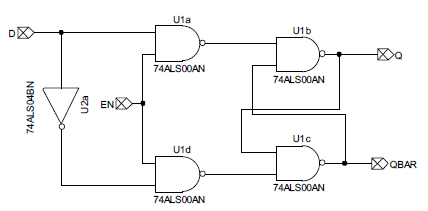
\includegraphics[scale=0.4]{D_latch.png}
	\caption{Schema circuitale del Flip-Flop D-Latch.}
	\label{f:D-Latch}
\end{figure}

\begin{figure}[h]
	\centering
	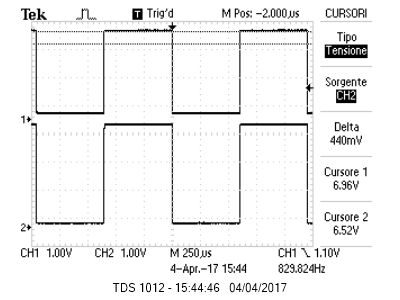
\includegraphics[scale=0.4]{Q.png}
	\caption{Il segnale in alto è l'ingresso ,mentre l'atro l'uscita Q.}
	\label{f:Q}
\end{figure}

\begin{figure}[h]
	\centering
	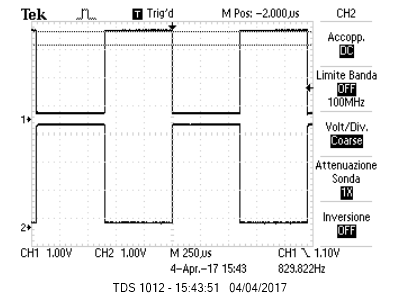
\includegraphics[scale=0.4]{Qbar.png}
	\caption{Il segnale in alto è l'ingresso ,mentre l'atro l'uscita Qbar.}
	\label{f:Qbar}
\end{figure}

\begin{figure}[h]
	\centering
	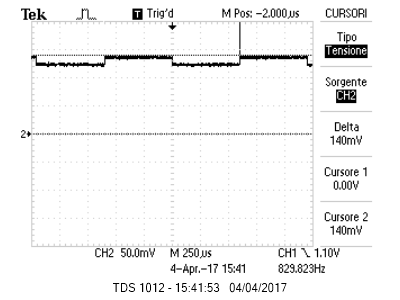
\includegraphics[scale=0.4]{Qbar_enable_basso.png}
	\caption{Uscita Qbar con ENABLE nel livello basso}
	\label{f:Qbar_enable_basso}
\end{figure}

\begin{figure}[h]
	\centering
	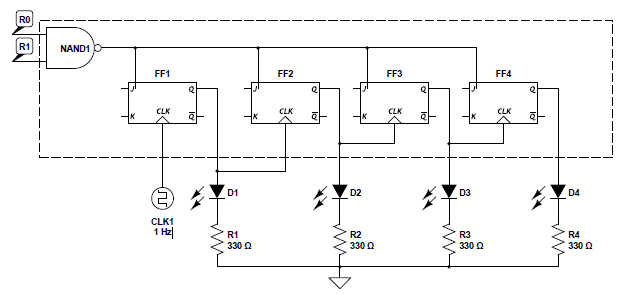
\includegraphics[scale=0.4]{divisore_freq.png}
	\caption{}
	\label{f:contatore}
\end{figure}

\begin{figure}[h]
	\centering
	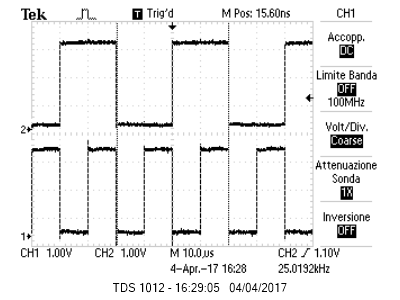
\includegraphics[scale=0.4]{Qa_vs_clock.png}
	\caption{Il segnale in basso è il clock, mentre quello in alto è  l'ingresso del diodo D1.}
	\label{f:Qa_vs_clock}
\end{figure}

\begin{figure}[h]
	\centering
	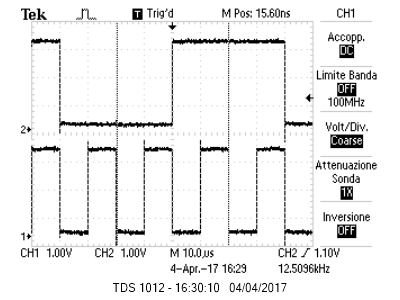
\includegraphics[scale=0.4]{Qb_vs_clock.png}
	\caption{Il segnale in basso è il clock, mentre quello alto è  l'ingresso del diodo D2}
	\label{f:Qb_vs_clock}
\end{figure}

\begin{figure}[h]
	\centering
	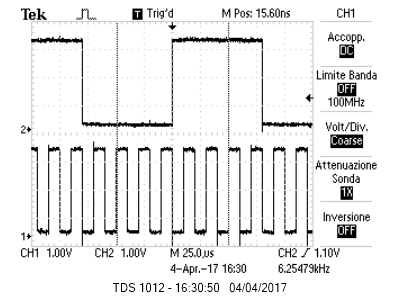
\includegraphics[scale=0.4]{Qc_vs_clock.png}
	\caption{Il segnale in basso è il clock, mentre quello alto è  l'ingresso del diodo D3}
	\label{f:Qc_vs_clock}
\end{figure}

\begin{figure}[h]
	\centering
	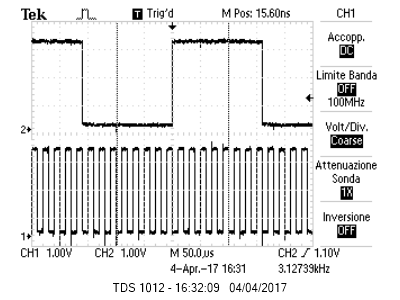
\includegraphics[scale=0.4]{Qd_vs_clock.png}
	\caption{Il segnale in basso è il clock, mentre quello alto è  l'ingresso del diodo D4}
	\label{f:Qd_vs_clock}
\end{figure}

\begin{figure}[h]
	\centering
	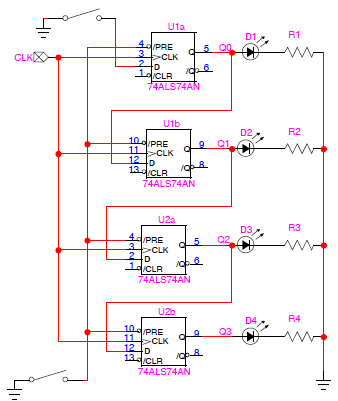
\includegraphics[scale=0.6]{shift_register.png}
	\caption{Schema circuitale usato per realizzare uno shift register con D-Latch}
	\label{f:shift_register}
\end{figure}


\begin{figure}[h]
	\centering
	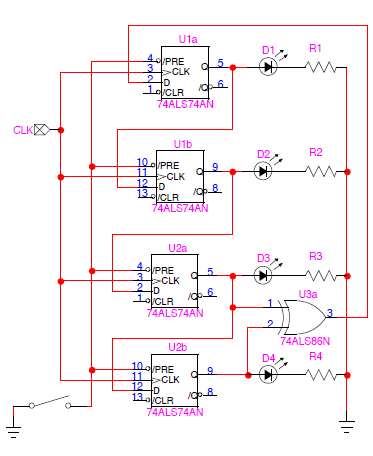
\includegraphics[scale=0.6]{gen_pseudocasuali.png}
	\caption{Schema circuitale usato per realizzare un generatore di sequenze pseudo casuali}
	\label{f:gen_pseudocasuali}
\end{figure}

\begin{figure}[h]
	\centering
	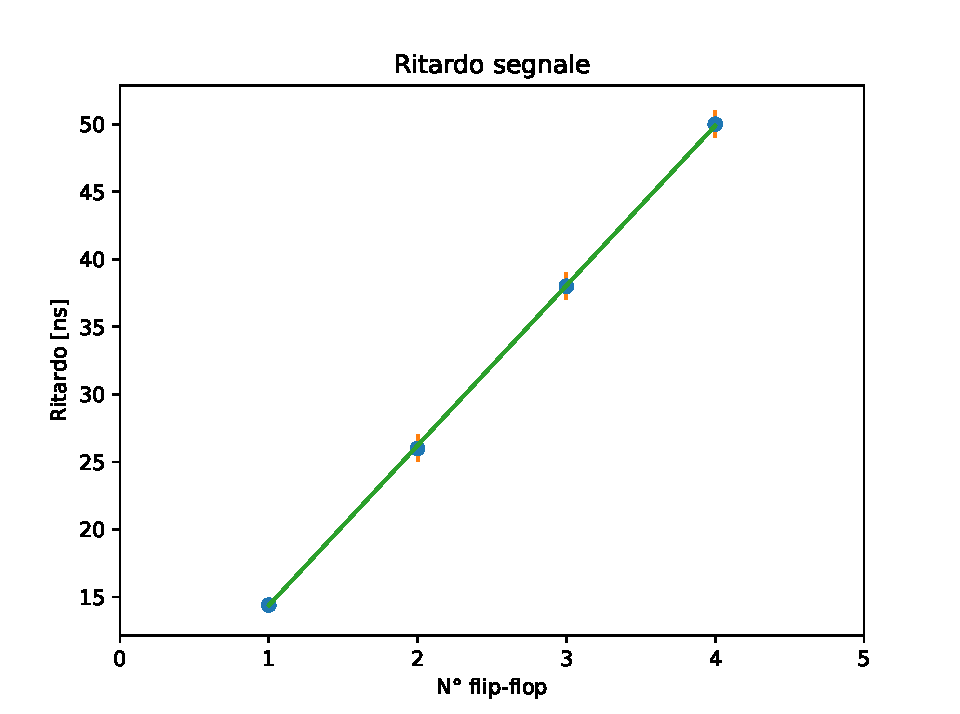
\includegraphics[scale=0.6]{lineare_ritardi.pdf}
	\caption{Ritardi delle uscite Q1,Q2,Q3,Q4 rispetto al CLOCK.}
	\label{f:ritardo}
\end{figure}